\chapter{Основы алгебры логики}
\label{ch:alog}

Даётся неформальное введение в алгебру логики. Этот минимум знаний необходим для успешного освоения следующих тем. Для углублённого изучения алгебры логики и булевых функций рекомендуются \cite{bib:yablonsky:discreteintro,bib:novic:discrmathprogrammer}.

\section{Логические функции}

Любое логическое выражение является \emph{истинным} или \emph{ложным}. Для удобства обозначим истину символом $1$, а ложь --- символом $0$. Выполнен очевидный переход к двоичным цифрам --- битам. Именно алгебра логики лежит в основе современных вычислительных устройств, в подавляющем большинстве которых числа представлены именно в двоичной системе счисления (см. раздел \ref{s:ch:ss:binaryNS}). 

\emph{Логическими} функциями называются функции вида 
    \begin{equation}
        \label{eq:ch:alog:binfunc}
        f(x_1,\ldots,x_n),
    \end{equation}
где, как аргументы $x_i$, так и функция принимают значение либо $0$, либо $1$.

Логическую \emph{функцию} \eqref{eq:ch:alog:binfunc} удобно задать с помощью \emph{таблицы истинности}:
\[
    \begin{array}{cccc|c}
        x_1 &\cdots&x_{n-1} &x_n&f(x_1,\cdots,x_{n-1},x_n)\\
        \hline
        0   &\cdots&0       &0  &y_0=f(0,\cdots,0,0)\\
        0   &\cdots&0       &1  &y_1=f(0,\cdots,0,1)\\
        0   &\cdots&1       &0  &y_2=f(0,\cdots,1,0)\\
        0   &\cdots&1       &1  &y_3=f(0,\cdots,1,1)\\
        \cdots   &\cdots&\cdots       &\cdots  &\cdots\\
        1   &\cdots&1       &1  &y_{2^n-1}=f(1,\cdots,1,1)\\
        \hline
    \end{array}
\]

Оценим количество всех возможных функций для заданного количества аргументов. Если зафиксировать количество аргументов $n$ логической функции \eqref{eq:ch:alog:binfunc}, то можно рассматривать их как $n$-разрядное двоичное число $X=(x_n\cdots x_1)_2$. Всех возможных вариантов аргументов, очевидно, $2^n$. При этом логическую функцию \eqref{eq:ch:alog:binfunc} можно рассматривать как функцию $f(X)$ одного целочисленного аргумента $X$, который изменяется в пределах от $0$ до $2^n-1$. Каждому значению $X$ будет соответствовать  либо $0$-е, либо $1$-е значение $y_X=f(X)$. Это значит, что саму функцию можно рассматривать как $2^n$-разрядное двоичное число $(y_{2^n-1}\cdots y_0)_2$. Всего таких чисел, а стало быть и функций, будет
\[
    2^{2^{n}}.
\]

Для всех функций, рассмативаемых ниже, приводится также условные графические обозначения соответствующих им элементов логических схем.

Логических функций одного аргумента всего $2^{2^{1}}=4$. Первые три из перечисленных практического интереса не представляют.
\begin{enumerate}
    \item \emph{Константа нуля} для любого аргумента вернёт $0$: $f(x)=0$.
    \item \emph{Константа единицы} для любого аргумента вернет $1$: $f(x)=1$, 
    \item \emph{Тождественная функция} вернет значение аргумента: $f(x)=x$.
    \item \emph{Отрицание}:
        \[
            \begin{array}{ccc}
                \begin{array}{c|c}
                    x_1&\textit{не}(x_1)\\
                    \hline
                    0&1\\
                    1&0\\
                    \hline
                \end{array}
                &&
                \raisebox{-.7\height}{
                    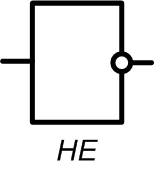
\includegraphics[width=.17\textwidth]{fig/not}
                }
            \end{array}
        \]
        <<$\textit{не}(x)$>> также обозначается: <<$\lnot x$>>, <<$\overline{x}$>>.
\end{enumerate}

Из $2^{2^2}=16$ функций двух аргументов далее рассматриваются лишь те, которые понадобятся в дальнейшем. 
\begin{itemize}
    \item $\textit{и}(x_1,x_2)$. Конъюнкция (\textit{И}, \textit{AND}). 
    \[
        \begin{array}{ccc}
            \begin{array}{cc|c}
                x_1&x_2&\textit{и}(x_1,x_2)\\
                \hline
                0&0&0\\
                0&1&0\\
                1&0&0\\
                1&1&1\\
                \hline
            \end{array}
            &&
            \raisebox{-.7\height}{
                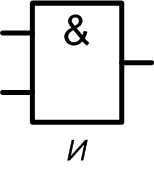
\includegraphics[width=.17\textwidth]{fig/and}
            }
        \end{array}
    \]
    
    Конъюнкция истинна только тогда, когда истинны оба аргумента. <<$\textit{и}(x,y)$>> также обозначается <<$x\land y$>>, <<$x \& y$>>, <<$x \cdot y$>> или <<$xy$>>.

    \item $\textit{или}(x_1,x_2)$. Дизъюнкция, \textit{ИЛИ}, \textit{OR}.
    \[
        \begin{array}{ccc}
            \begin{array}{cc|c}
                x_1&x_2&\textit{или}(x_1,x_2)\\
                \hline
                0&0&0\\
                0&1&1\\
                1&0&1\\
                1&1&1\\
                \hline
            \end{array}
            &&
            \raisebox{-.7\height}{
                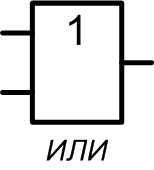
\includegraphics[width=.17\textwidth]{fig/or}
            }
        \end{array}
    \]
    
    Дизъюнкция ложна только тогда, когда ложны оба аргумента. <<$\textit{или}(x,y)$>> также обозначается <<$x \lor y$>>.

    \item $\textit{xor}(x_1,x_2)$. <<Исключающее или>>, <<сложение по модулю два>>, \textit{XOR} --- eXclusive OR.
    \[
        \begin{array}{ccc}
            \begin{array}{cc|c}
                x_1&x_2&\textit{xor}(x_1,x_2)\\
                \hline
                0&0&0\\
                0&1&1\\
                1&0&1\\
                1&1&0\\
                \hline
            \end{array}
            &&
            \raisebox{-.7\height}{
                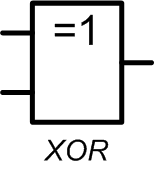
\includegraphics[width=.17\textwidth]{fig/xor}
            }
        \end{array}
    \]
    
    \emph{Исключающим или} функция названа потому, что $\textit{xor}(x_1,x_2)$ истинна, если истинно $x_1$ \emph{или} истинно $x_2$, \emph{но не} оба сразу. Проще запомнить эту функцию, как результат арифметического сложения двух бит с отброшенным переносом. <<$\textit{xor}(x,y)$>> также обозначается: <<$x \oplus y$>>.

    \item $\textit{если-то}(x_1,x_2)$. Импликация, \textit{ЕСЛИ-ТО}.
    \[
        \begin{array}{cc|c}
            x_1&x_2&\textit{если-то}(x_1,x_2)\\
            \hline
            0&0&1\\
            0&1&1\\
            1&0&0\\
            1&1&1\\
            \hline
        \end{array}
    \]
    
    Импликация является аналогом высказывания <<если $x_1$, то $x_2$>>. Оно ложно лишь тогда, когда посылка $x_1$ истинна, а следствие $x_2$ ложно. <<$\textit{если-то}(x,y)$>> также обозначается: <<$x \to y$>>.
    
    \item $\textit{и-не}(x_1,x_2)$. Штрих Шеффера, \textit{И-НЕ}.
    \[
        \begin{array}{ccc}
            \begin{array}{cc|c}
                x_1&x_2&\textit{и-не}(x_1,x_2)\\
                \hline
                0&0&1\\
                0&1&1\\
                1&0&1\\
                1&1&0\\
                \hline
            \end{array}
            &&
            \raisebox{-.7\height}{
                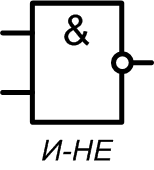
\includegraphics[width=.17\textwidth]{fig/notAnd}
            }
        \end{array}
    \]
    
    <<$\textit{и-не}(x,y)$>> также обозначается: <<$x\mid y$>>.

    \item $\textit{или-не}(x_1,x_2)$. Стрелка Пирса, \textit{ИЛИ-НЕ}.
    \[
        \begin{array}{ccc}
            \begin{array}{cc|c}
                x_1&x_2&\textit{или-не}(x_1,x_2)\\
                \hline
                0&0&1\\
                0&1&0\\
                1&0&0\\
                1&1&0\\
                \hline
            \end{array}
            &&
            \raisebox{-.7\height}{
                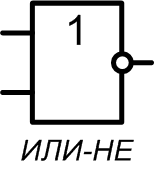
\includegraphics[width=.17\textwidth]{fig/notOr}
            }
        \end{array}
    \]
    
    <<$\textit{или-не}(x,y)$>> также обозначается: <<$x\uparrow y$>>.
\end{itemize}

В заключение упомянем такие достойные функции двух аргументов, как \emph{константы нуля} и \emph{единицы}, \emph{эквивалентность}, \emph{штрих Шеффера} и \emph{стрелку Пирса}. Их рассматривать не будем. 

Не имеет смысла рассматривать \emph{функции} трех и большего количества аргументов, в силу того, что их можно выразить \emph{формулой}, сконструированной из функций одного и/или двух аргументов.


\section{Формулы}

Формулой будем называть выражение 
\begin{equation}
    \label{eq:ch:alog:binform}
    f(t_1,\ldots,t_n),
\end{equation}
где аргумент $t_i$ --- подформула, т.е. либо аналогичного вида формула, либо переменная, принимающая одно из значений $0$, либо $1$.

Прежде чем найти значение формулы, нужно найти значения подформул, стоящих в аргументах.

\begin{exampl} Задача. Найти значение формулы 
\[
    \textit{или}(0,\textit{и}(\textit{не}(1), 1)).
\]
\end{exampl}
\begin{proof}[Решение] 
\(
    \textit{или}(0,\textit{и}(\textit{не}(1), 1))\Rightarrow
    \textit{или}(0,\textit{и}(0, 1))\Rightarrow
    \textit{или}(0,0)\Rightarrow 0
\)
\end{proof}

Функции произвольного количества аргументов можно конструировать на основе вышеназванных функций одного и двух аргументов. 
    \begin{exampl}\label{ex:ch:alog:f3arg} Функция трёх аргументов 
    \[
        g(x_1,x_2,x_3)=\textit{или}(x_1,\textit{и}(\textit{не}(x_2), x_3))
    \]
    задана формулой. Соответствующая формуле логическая схема приведена на рисунке \ref{fig::alog:formulae}.
\end{exampl}

\begin{figure}[!ht]
    \centering
    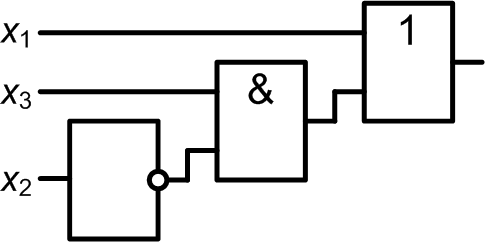
\includegraphics[width=.42\textwidth]{fig/formulae}
    \caption{Логическая схема $g(x_1,x_2,x_3)=\textit{или}(x_1,\textit{и}(\textit{не}(x_2), x_3))$}
    \label{fig::alog:formulae}
\end{figure} 

Кроме того, на практике всегда в формулах вместо обозначений функций используют символы \emph{операции}, например:
\begin{itemize}
    \item вместо <<$\textit{не}(x)$>> пишут <<$(\lnot x)$>> или <<$(\bar{x})$>>;
    \item вместо <<$\textit{и}(x,y)$>> пишут <<$(x \land y)$>>, <<$(x \& y)$>>,  <<$(x \cdot y)$>> или  <<$(xy)$>>;
    \item вместо <<$\textit{или}(x,y)$>> пишут <<$(x \lor y)$>>;
    \item вместо <<$\textit{xor}(x,y)$>> пишут <<$(x \oplus y)$>>;
    \item вместо <<$\textit{если-то}(x,y)$>> пишут <<$(x \to y)$>>.
\end{itemize}

Задавая приоритет операций (выше они перечислены в порядке убывания приоритета), лишние скобки опускают.
\begin{exampl} 
    <<$\lnot x\lor y\land z$>> то же самое, что <<$(\lnot x)\lor (y\land z)$>>.
\end{exampl}

\begin{exampl}
    Функция $g(x_1,x_2,x_3)$ из примера \ref{ex:ch:alog:f3arg}:
    \[
        g(x_1,x_2,x_3) = x_1 \lor \lnot x_2 \land x_3
    \]
\end{exampl}


\section{Основной логический базис}

Функции \emph{И}, \emph{ИЛИ}, \emph{НЕ} составляют \emph{основной логический базис}. Любую функцию можно выразить формулой на их основе. Эти логические связки часто используются в обыденной жизни.

Принцип конструирования любой функции в основном логическом базисе демонстрируется следующим примером.

\begin{exampl} Задача. Представить функцию $f(x_1,x_2,x_3)$ в основном логическом базисе.
    \[
        \begin{array}{ccc|c}
            x_1&x_2&x_3&f(x_1,x_2,x_3)\\
            \hline
            0&0&0&0\\
            0&0&1&0\\
            0&1&0&1\\
            0&1&1&0\\
            1&0&0&0\\
            1&0&1&0\\
            1&1&0&1\\
            1&1&1&0\\
            \hline
        \end{array}    
    \]
\end{exampl}
\begin{proof}[Решение]
    На наборе $x_1=0$, $x_2=1$, $x_3=0$ функция $f(x_1,x_2,x_3)$ должна равняться единице. При этом видно, что функция $f_2(x_1,x_2,x_3)=\overline{x_1}\land x_2 \land\overline{x_3}$ равняется единице только на этом наборе. $f(x_1,x_2,x_3)$ также должна равняться $1$ на наборе $x_1=1$, $x_2=1$, $x_3=0$. $f_6(x_1,x_2,x_3)=x_1\land x_2 \land\overline{x_3}$. Стало быть\footnote{Конечно, это решение можно оптимизировать. Вдумавшись, можно видеть, что от $x_1$ функция не зависит: $f(x_1,x_2,x_3)=x_2 \land\overline{x_3}$. Такое представление называется ДНФ --- дизъюнктивная нормальная форма. Оптимизация формул здесь не рассматривается} $f(x_1,x_2,x_3)=f_2(x_1,x_2,x_3)\lor f_6(x_1,x_2,x_3)=(\overline{x_1}\land x_2 \land\overline{x_3})\lor(x_1\land x_2 \land\overline{x_3})$.
\end{proof}

Оказывается, что основной логический базис избыточен. Например, функцию \emph{И} можно выразить через функции \emph{ИЛИ} и \emph{НЕ}. Действительно $x_1\land x_2 = \overline{\overline{x_1}\lor\overline{x_1}}$, в чём нетрудно убедиться непосредственной проверкой:
\[
    \begin{array}{c|cc|c}
        x_1\land x_2&x_1&x_2&\overline{\overline{x_1}\lor\overline{x_1}}\\
        \hline
        0&0&0&0\\
        0&0&1&0\\
        0&1&0&0\\
        1&1&1&1\\
        \hline
    \end{array}
\]

Впрочем, чтобы образовать базис, достаточно и одной функции. Например, функции \emph{стрелка Пирса} или \emph{штрих Шеффера} в одиночку образуют базис. И любую функцию можно выразить через одну из них. 

Для того, чтобы это доказать, достаточно выразить, например функции \textit{НЕ} и \textit{ИЛИ} через стрелку Пирса (см. схему на рисунке \ref{fig::alog:orByNotOr}):
\begin{itemize}
    \item \textit{НЕ}: $\lnot x=x\uparrow x$;
    \item \textit{ИЛИ}: $x\lor y=\lnot(x\uparrow y)=(x\uparrow y)\uparrow(x\uparrow y)$;
\end{itemize}

\begin{figure}[!ht]
    \centering
    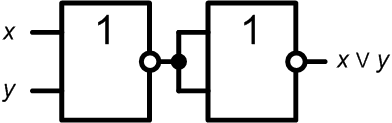
\includegraphics[width=.45\textwidth]{fig/orByNotOr}
    \caption{$x\lor y=\lnot(x\uparrow y)=(x\uparrow y)\uparrow(x\uparrow y)$}
    \label{fig::alog:orByNotOr}
\end{figure} 

Выбор базиса и эффективное упрощение формул в нём сильно влияют на стоимость создаваемых в итоге вычислительных устройств.


\section*{Задания}
\addcontentsline{toc}{section}{Задания}


\paragraph{Задания базового уровня}

\begin{enumerate}
    \item Доказать или опровергнуть утверждения:
    \begin{enumerate}
        \item $\overline{\overline{x}}=x$;
        \item $x\oplus 1=\overline{x}$;
        \item $x\oplus 0=x$;
        \item $x\oplus x=0$;
        \item $x\lor y = y\lor x$;
        \item $x\land y = y\land x$;
        \item $x\to y = \overline{x}\lor y$;
        \item $(x\lor y)\lor z = x\lor(y\lor z)$;
        \item $x\land (y\lor z) = (x\land y)\lor(x\land z)$;
        \item $x\lor (y\land z) = (x\lor y)\land(x\lor z)$;
        \item $\overline{x\lor y}=\overline{x}\land\overline{y}$;
    \end{enumerate}
    
    \item Сколько существует функций четырёх аргументов? Пяти?
    
    \item Выразить функцию \emph{ИЛИ} через функции \emph{И}, \emph{НЕ}.

    \item Выразить импликацию в основном логическом базисе.
    
    \item Построить таблицу истинности для функции:
    \begin{enumerate}
        \item $f(x)=x\to x$;
        \item $f(x,y)=\overline{\overline{x}\lor y}$;
        \item $f(x,y,z)=(\overline{x}\lor y)\land(\overline{y}\lor z)$.
    \end{enumerate}
    
    \item Записать формулу, используя знаки операций:
    \begin{enumerate}
        \item $\textit{или}(\textit{или}(a,b),\textit{и}(c,d))$;
        \item $\textit{не}(\textit{или}(a,\textit{или}(\textit{не}(b),c)))$;
        \item $\textit{xor}(\textit{не}(\textit{и}(c,\textit{если-то}(a,b))),d)$.
    \end{enumerate}
    
    Лишние скобки следует опустить.

    \item\label{en:ch:alog:logicVentils} На функциональных схемах логические элементы основного логического базиса изображаются так
    \begin{center}
        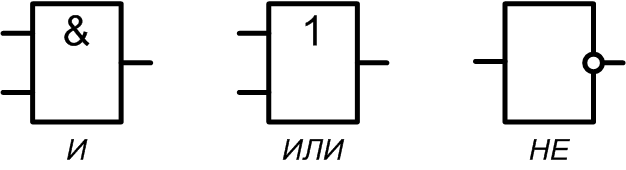
\includegraphics[width=.5\textwidth]{fig/logicVentils}
    \end{center}
    
    Нарисовать схему, соответствующую формуле:
    \begin{enumerate}
        \item $(x\lor y\lor z)\land\overline{x}$;
        \item $x\lor\overline{(y\land z)}$;
        \item $x\land\overline{\overline{y}\lor z}$;
        \item $\overline{x\land\overline{y\land\overline{z}}}$;
        \item $x\land y\land z\lor(\overline{x\land y})$;
        \item $x\oplus y$;
        \item $x\to (y\to z)$.
    \end{enumerate}
    
    Записать формулу, перейдя от знаков операций к обозначениям функций. Например, $x\land y$ соответствует $\textit{и}(x,y)$.
    
    \item\label{en:ch:alog:psum} Полусумматором называется логическая схема, принимающая на входе две двоичные цифры-слагаемые текущего разряда, а на выходе формирующая результат и перенос в следующий разряд. Задать формулы для результата и переноса в основном логическом базисе, и нарисовать схему из элементов, представленных в задании \ref{en:ch:alog:logicVentils} данного блока.
    
    \item Двоичным сумматором называется логическая схема, принимающая на входе две двоичные цифры-слагаемые текущего разряда и перенос из предыдущего разряда, а на выходе формирующая результат и перенос в следующий разряд. Сформировать сумматор на основе полусумматоров (см. задание \ref{en:ch:alog:psum} данного блока) и функций основного логического базиса. Сформировать из сумматоров схему, складывающую $4$-х разрядные числа.
    
\end{enumerate}


\paragraph{Программирование}
\begin{enumerate}
    \item Компьютерная память хранит двоичные данные блоками бит фиксированного размера --- \emph{байтами}. Будем считать, что байт --- это восемь бит. Процессоры также поддерживают логические операции, в которых в качестве оперендов выступают байты, при этом операции выполняются над битами соответствующих разрядов. Рассмотрим некоторые операторы языка C. 
    \begin{center}
        \begin{tabular}{c|l}
            \hline\hline
            Оператор C & Действие оператора\\
            \hline\hline
            \verb"x=y"  &Присвоить переменной \verb"x" значение \verb"y"\\
            \verb"x==y" &Сравнить значения переменных \verb"x" и \verb"y"\\
            \verb"~x"   &Битовое \emph{НЕ}\\
            \verb"x|y"  &Битовое \emph{ИЛИ}\\
            \verb"x&y"  &Битовое \emph{И}\\
            \verb"x^y"  &Битовое \emph{XOR}\\
            \verb"x<<n" &Сдвиг значения \verb"x" на \verb"n" бит влево\\
            \verb"x>>n" &Сдвиг значения \verb"x" на \verb"n" бит вправо\\
            \hline
        \end{tabular}
    \end{center}
    
    В качестве примера приведём фрагмент программы:
\begin{verbatim}    
    x  = 60; //00111100b
    y  = 90; //01011010b
    z1 = ~x;
    z2 = x|y;
    z3 = x&y;
    z4 = x^y;
    z5 = x<<1;
    z6 = x>>2;
\end{verbatim}

    И результаты его выполнения:
    \begin{center}
        \begin{tabular}{lcccccccccc}
                     &&\small{7}&\small{6}&\small{5}&\small{4}&\small{3}&\small{2}&\small{1}&\small{0}& \\ \cline{3-10}
            \verb"x"    &\multicolumn{1}{c|}{}  &0&0&1&1&1&1&0&0&\multicolumn{1}{|c}{}\\ \cline{3-10}
            \verb"y"    &\multicolumn{1}{c|}{}  &0&1&0&1&1&0&1&0&\multicolumn{1}{|c}{}\\ \cline{3-10}
            \\ \cline{3-10}
            \verb"z1 = ~x"   &\multicolumn{1}{c|}{}  &1&1&0&0&0&0&1&1&\multicolumn{1}{|c}{}\\ \cline{3-10}
            \verb"z2 = x|y"  &\multicolumn{1}{c|}{}  &0&1&1&1&1&1&1&0&\multicolumn{1}{|c}{}\\ \cline{3-10}
            \verb"z3 = x&y"  &\multicolumn{1}{c|}{}  &0&0&0&1&1&0&0&0&\multicolumn{1}{|c}{}\\ \cline{3-10}
            \verb"z4 = x^y"  &\multicolumn{1}{c|}{}  &0&1&1&0&0&1&1&0&\multicolumn{1}{|c}{}\\ \cline{3-10}
            \verb"z5 = x<<1" &\multicolumn{1}{c|}{}  &0&1&1&1&1&0&0&0&\multicolumn{1}{|c}{}\\ \cline{3-10}
            \verb"z6 = x>>2" &\multicolumn{1}{c|}{}  &0&0&0&0&1&1&1&1&\multicolumn{1}{|c}{}\\ \cline{3-10}
        \end{tabular}
    \end{center}
    
    Задания.
    \begin{enumerate}
        \item Чему равно \verb"(7&3)|12"?
        \item Чему равно \verb"(90&0xF)<<(~0xFC)"?
        \item Напишите программу, записывающую значение $(1010)_2$ в старшие $4$ бита байта \verb"x".
        \item Напишите программу, проверяющую установлен ли \verb"n"-й бит в байте \verb"x"?
        \item Напишите программу, устанавливающую \verb"n"-й бит в байте \verb"x" в $1$.
        \item Напишите программу, сбрасывающую \verb"n"-й бит в байте \verb"x" в $0$.
        \item Напишите программу, меняющую местами старшую и младшую тетрады\footnote{Тетрада --- четыре бита} байта.
        \item Напишите программу, выполняющую циклический сдвиг байта \verb"x" на \verb"n" бит вправо.
        \item Напишите программу, инвертирующую младшую тетраду байта \verb"x".
    \end{enumerate}
\end{enumerate}


\paragraph{Философия}
\begin{enumerate}
    \item Функция \emph{штрих Шеффера}, называемая также \emph{И-НЕ}, образует базис. Обозначается она символом операции $x\mid y$:
    \[
        \begin{array}{cc|c}
            x_1&x_2&x_1\mid x_2\\
            \hline
            0&0&1\\
            0&1&1\\
            1&0&1\\
            1&1&0\\
            \hline
        \end{array}
    \]
    выразить через неё функции основного логического базиса.

    \item Функция \emph{стрелка Пирса}, называемая также \emph{ИЛИ-НЕ}, образует базис. Обозначается она символом операции $x\uparrow y$:
    \[
        \begin{array}{cc|c}
            x_1&x_2&x_1\uparrow x_2\\
            \hline
            0&0&1\\
            0&1&0\\
            1&0&0\\
            1&1&0\\
            \hline
        \end{array}
    \]
    выразить через неё функции основного логического базиса.
    
\end{enumerate}

